\documentclass[a4paper]{scrartcl}
%\usepackage{tikz}
\usepackage[
typ={ib},
fach=Informatik,
farbig
]{schule}
%\hypersetup{hidelinks}


%\usepackage{ctable}
%
%´\usepackage[default]{fontsetup}

%\usepackage[default]{fontsetup}
\usepackage{fontspec}
\usepackage{fourier-otf}

\usepackage{float}
\usetikzlibrary{arrows,calc,positioning}
%\setmonofont{FiraCode-Regular}[
%Contextuals=Alternate % Activate the calt feature
%]
%\usepackage{newunicodechar}
%\newunicodechar{^^^^2588}{█}
%\newunicodechar{█}{█}
%\setmonofont{Fira Code}
%\usepackage{amsmath}
%\usepackage{amssymb}
%\setmonofont{Ubuntu Mono Regular}[Scale=0.9]
%\usepackage{pmboxdraw}
%\usepackage{cascadia-code}
\usepackage[scale = 0.1]{jetbrainsmono-otf}
%\usepackage{cascadiamono-otf}
%\setmonofont{CascadiaMono-SemiLight}[]
\setmonofont[Scale = MatchLowercase]{jetbrainsmono-light}
%\newunicodechar{2588}{█}
%\newunicodechar{█}{\pmboxdrawuni{2588}}

\usepackage{scrlayer-scrpage}
\ifoot{% TODO: \usepackage{graphicx} required
	
	
\includegraphics[width=0.35\linewidth]{GHSE-Logo}
	
}

\usepackage[ngerman]{babel} 
\usepackage{tikz}
\usepackage{shellesc}
\usepackage{minted}
	\usepackage{url}
\usepackage{microtype}	
\usepackage[font=tiny,labelfont=bf]{caption}
\usepackage{xcolor}
\usepackage{color}
\usepackage{fancyvrb}
\date{}
\usetikzlibrary{positioning} 
\title{HTTP-Kontrollelemente}
\begin{document}
\maketitle
\section{Links}

Link-Elemente haben in HTML die folgende Form:
\begin{minted}{HTML}
 <a href="http://www.github.com/login"> Github-Login </a> 
\end{minted}

Der Wert des Attributs \mintinline{html}|href| ist eine URL. Beim Klicken auf den Link wird eine HTTP-GET-Anfrage an diese Adresse geschickt.
\footnotesize
\begin{Verbatim}
┌────────────────────────┐      ┌─HTTP REQUEST────────────────┐
│ BROWSER              X │      │                             │
├────────────────────────┤      │ GET /login HTTP2            │
│ ┌────────────────────┐ │      │ Host: github.com            │
│ │ Github-Login       │ │      │ Accept: text/html ...       │
│ └────────────────────┘ │      └─────────────────────────────┘
│                    ────┼───────────┐
│                        │           │
│                        │           │
└────────────────────────┘           │
                              ┌──────▼──────┐
                              │   H T T P   │
                              │ S E R V E R │
                              └──────┬──────┘
┌────────────────────────┐           │
│ BROWSER              X │           │
├────────────────────────┤           │
│                        │           │
│ Sign in to github      │ ◀─────────┘
│                        │
│                        │      ┌─HTTP RESPONSE───────────────┐
│ ────────────────────── │      │                             │
│  ....                  │      │ HTTP/2 200                  │
│                        │      │ ...                         │
└────────────────────────┘      │ <html lang="en">            │
                                │ ....                        │
                                │ <title>Sign in to github    │
                                └─────────────────────────────┘
\end{Verbatim}

\normalsize
Wenn der Browser die Antwort erhalten hat, ersetzt er seinen gesamten momentanen Inhalt durch den HTML-Code in der Antwort des HTTP-Servers.


Ein Link kann auch nur aus einem Pfad bestehen.
Man spricht dann von einer relativen Adresse.

\begin{minted}{HTML}
 <a href="/login"> Sign in </a> 
\end{minted}

Wenn der Link oben auf der Seite \texttt{github.com} steht, wird beim Klicken auf diesen Link wird eine HTTP-GET-Anfrage an \texttt{github.com/login} geschickt.

\section{Formulare}

Auch mit Formularen können HTTP-Anfragen an einen Server geschickt werden.
Dabei wird ebenfalls der Browserinhalt durch den HTML-Code in der Antwort des HTTP-Servers ersetzt.
Die eingegebenen Daten werden mit der Anfrage vom Client zum Server übertragen

% TODO: \usepackage{graphicx} required
\begin{figure}[H]
\centering
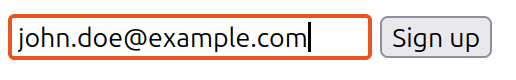
\includegraphics[width=0.5\linewidth]{formular}
\caption{Formular}
\label{fig:formular}
\end{figure}
\scriptsize
\begin{Verbatim}
┌────────────────────────┐      ┌─HTTP REQUEST────────────────┐
│ BROWSER              X │      │                             │
├────────────────────────┤      │ POST /signUpForNewsletter   │
│                        │      │ Host: hypermedia.systems    │
│ SIGN UP                │      │ ...                         │
│ ┌────────────────────┐ │      │ email=joe@example.com       │
│ │ joe@example.com    │ │      └─────────────────────────────┘
│ └────────────────────┘ │
│ ┌─────────┐        ────┼───────────┐
│ │ Sign up │            │           │
│ └─────────┘            │           │
└────────────────────────┘           │
                              ┌──────▼──────┐
                              │   H T T P   │
                              │ S E R V E R │
                              └──────┬──────┘
┌────────────────────────┐           │
│ BROWSER              X │           │
├────────────────────────┤           │
│                        │           │
│ THANK YOU FOR SIGNING  ◀───────────┘
│ UP                     │
│                        │      ┌─HTTP RESPONSE───────────────┐
│                        │      │                             │
│                        │      │ 201 Created                 │
│                        │      │ ...                         │
└────────────────────────┘      │ <h1>Thank you for signing   │
                                │ up</h1>                     │
                                └─────────────────────────────┘
\end{Verbatim}
\normalsize

Ein Formular kann folgendermaßen erstellt werden:

\begin{minted}{HTML}
<form action="/signUpForNewsletter" method="post" >
    <input name="email" value="" />
    <button type="submit"> Sign up </button>
</form>
\end{minted}

Das  \mintinline{html}|form|-Element hat zwei Attribute.

\begin{table}[H]
\begin{tabular}{ll}
Attribut & Bedeutung \\
\hline
\texttt{action} & Adresse an die, die  HTTP-Abfrage mit den eingetragenen Daten geschickt werden soll \\

\texttt{method} & HTTP-Methode, die zum Senden der Daten genutzt werden soll.
\\
 & Nur \texttt{GET} und \texttt{POST} können verwendet werden.\\


\end{tabular}
\end{table}



In dem \mintinline{html}|form|-Element befindet sich ein \mintinline{html}|Input|-Element.
Dieses hat auch zwei Attribute.

\begin{itemize}
\item{name}: Der Name unter dem der eingetragene Wert verschickt wir. Im Beispiel oben ist der Wert dieses Attributs \texttt{E-Mail}. Deshalb wird nach der Eingabe von \texttt{joe@example.com} beim Versenden des Formulars, die Information \texttt{email=joe@example.com} mitgeschickt. Dabei handelt es sich um einen \texttt{Formparameter}
\item {value} ist der Wert, der direkt nach dem Laden des Elements in dem Textfeld steht. In unserem HTML-Code steht \mintinline{html}|value=""|. Deshalb ist das Textfeld beim Laden der Seite leer.
\end{itemize}


Weil der \mintinline{html}|button| sich im Formular befindet und den Typ \texttt{submit} hat, kann er verwendet werden, um das Formular abzuschicken.

\section{Weitere wichtige Einstellungsmöglichkeiten von Input-Elementen}

Mit dem Attribut \texttt{autofocus} kann festgelegt werden, dass ein \texttt{input} ausgewählt ist, nachdem es geladen wurde.
Der Benutzer muss also nicht erst in das Textfeld klicken, um etwas zu schreiben.

\begin{minted}{HTML}
<input autofocus name="email" value="" />
\end{minted}


Mit dem Attribut \texttt{placeholder} kann angezeigt werden, was in dem Textfeld steht, bis etwas eingegeben wurde.

\begin{minted}{HTML}
<input placeholder="Type in your email" name="email" value="" />
\end{minted}

\begin{figure}[H]
\centering
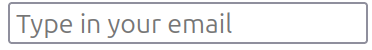
\includegraphics[width=0.5\linewidth]{placeholder}
\caption{Platzhalter}
\label{fig:placeholder}
\end{figure}

\end{document}
